\chapter{Definiciones y acrónimos}
\label{Appendix:1}

\chapterquote{Saber dónde encontrar la información y cómo usarla. Ese es el secreto del éxito} {Albert Einstein}
-

Dedicaremos este apéndice a la explicación de conceptos en más extensión, ya sea conceptos más generales o la explicación del significado de los acrónimos de esta memoria.

\section{Definiciones}

Separaremos este apartado, de la misma manera que se ha hecho en otras partes de la memoria, en los tres grandes elementos que conforman esta memoria, definiciones referentes a datos, a nubes y a Inteligencia artificial.

\subsection{Referente a datos}

\begin{enumerate}
	\item El gobierno de España define los \textbf{datos de alto valor} \label{def1}  como “documentos cuya reutilización está asociada a considerables beneficios para la sociedad, el medio ambiente y la economía, en particular debido a su idoneidad para la creación de servicios de valor añadido, aplicaciones y puestos de trabajo nuevos, dignos y de calidad, y al número de beneficiarios potenciales de los servicios de valor añadido y aplicaciones basados en tales conjuntos de datos” Esta definición nos ofrece varias pistas sobre la manera en la que se prevé que se identifiquen esos conjuntos de datos de alto valor a través de una serie de indicadores que incluirían:
		\begin{itemize}
			\item Su potencial para generar beneficios sociales o medioambientales significativos.
			
			\item Su potencial para generar beneficios económicos y nuevos ingresos.
			
			\item Su potencial para generar servicios innovadores.
			
			\item Su potencial en cuanto a número de usuarios beneficiados, con atención particular a las PYMEs.
			
			\item Su capacidad para ser combinados con otros conjuntos de datos. \\
		\end{itemize}
		
	\item El \textbf{open government} \label{def2} o gobierno abierto es una forma de comunicación abierta, permanente y bidireccional entre la administración y los ciudadanos, basada en la transparencia por parte de la administración y la participación y colaboración con la sociedad civil y las empresas. Teniendo como punto clave el movimiento open data o datos abiertos, esta estructura y formatos abiertos permiten que los datos puedan reutilizarse proporcionando nuevos servicios a ciudadanos y empresas. En Europa sus orígenes se sitúan en la Directiva 2003/98/CE del Parlamento y del Consejo Europeos sobre el acceso y la reutilización de la información del sector público. \citep{OperGovernment2011}. \\
	
	\item El \textbf{Valor Público} se puede definir de muchas maneras y depende de la perspectiva de muchos autores:
	\label{def3} 
	\begin{itemize}
		\item[\textbullet] Para \textbf{Mark Moore}, su creador, consiste en conocer y satisfacer los deseos de la gente, un valor que lo público debe crear de forma análoga a como el sector privado crea valor económico. \citep{moore1995creating}
		\item[\textbullet] \textbf{Bozeman} lo define desde una perspectiva ciudadana como el consenso sobre los derechos y obligaciones de los ciudadanos, así como los principios sobre los que debe basarse el gobierno  \citep{bozeman2007public}. A menudo se refiere a ``valores públicos'', en plural, para destacar su diversidad, tema que seria llevado mas en profundidad por \textbf{Talbot}, que sugiere que a veces estos son contradictorios entre sí, reflejando la combinación de las diversas y conflictivas preferencias del público \citep{Talbot01012011}.
		\item[\textbullet] \textbf{Benington} lo vincula directamente con la ``esfera pública'', argumentando que el valor público no es solo lo que el público valora individualmente, sino también aquello que agrega valor a este espacio colectivo. \citep{Benington19032009}
		\item[\textbullet] Finalmente, \textbf{Timo Meynhardt} lo conceptualiza como un fenómeno relacional que surge de las percepciones. El valor público se crea en la relación entre el individuo y la sociedad, y depende de cómo las acciones de las organizaciones públicas impactan en la satisfacción de las necesidades básicas de las personas: morales, sociales, utilitarias y hedonistas  \citep{Meynhardt19032009}.
	\end{itemize}
	
	En un intento de resumirlo, el valor publico surge de las evaluaciones y percepciones que los individuos y colectivos realizan sobre cómo las acciones, servicios o políticas de las organizaciones públicas (y otras entidades) impactan en la satisfacción de sus diversas necesidades básicas dentro de un marco relacional que involucra a la esfera pública. Valor creado para y por la sociedad. \\


	\item Los \textbf{Datos Abiertos} \label{def4} se refieren a conjuntos de datos digitales que se publican bajo una filosofía de apertura, garantizando y facilitando el libre acceso, uso, modificación, reutilización y redistribución por parte de cualquier persona o entidad, en cualquier momento, lugar y con cualquier finalidad. Una parte especifica y importante para este trabajo son los Datos Abiertos de Gobierno, aquellos datos que se originan, producen, encargan o publican los gobiernos u organismos públicos en el ejercicio de sus funciones. Estos datos buscan, como fin último, fomentar la transparencia, la creación de valor público, la colaboración intersectorial y la resolución de problemas.
	
	La materialización de esta filosofía de apertura se concreta en requisitos técnicos y jurídicos específicos, cuya interpretación puede variar ligeramente entre las entidades que los definen. Desde el Grupo de Trabajo sobre Datos Abiertos ``Open Knowledge Foundation'' (OKF), “El conocimiento está abierto si alguien tiene la libertad de acceder a él, usarlo, modificarlo y compartirlo, sujeto, como máximo, a medidas que preserven su procedencia y su apertura” \citep{OpenKnowledgeFoundation}. El Portal Europeo de Datos y el ``Open Data Charter'', por su parte, enfatizan las condiciones de acceso y las libertades de uso, incluyendo la gratuidad y la ausencia de limitaciones, detallando la necesidad de características técnicas y jurídicas para que los datos sean libremente reutilizables y redistribuibles \citep{dataEuropaOpenData}, \citep{Open_Data_Charter}.
	Todo esto subraya la complejidad y la multifuncionalidad de los Datos abiertos como catalizador para la innovación y el desarrollo socioeconómico, con implicaciones legales y técnicas que deben ser gestionadas cuidadosamente para maximizar su potencial. \\
	
	\item Las \textbf{Tres olas del ``Open Data'' } \label{def5} representan las diferentes etapas evolutivas por las que ha transitado el movimiento de apertura de datos. 
	La \textbf{Primera Ola} (1990s-2000s) se fundamentó principalmente en Estados Unidos, dirigido a periodistas, abogados y activistas que solicitaban datos específicos bajo el modelo de ``derecho a saber'', enfrentando riesgos de secretismo gubernamental y requiriendo auditores de información. 
	La \textbf{Segunda Ola} (2000s-2010s) evolucionó hacia la apertura por defecto con alcance internacional, expandiendo su audiencia a agencias gubernamentales, empresas tecnológicas y organizaciones comunitarias,pero generando desafíos de privacidad que impulsaron la creación de portales de datos abiertos y responsables.
	La \textbf{Tercera Ola} (2010s-presente) representa la madurez del movimiento  con colaboración intersectorial y flujos transfronterizos, dirigiéndose a ONGs, instituciones académicas, pequeñas empresas y gobiernos, estableciendo marcos de responsabilidad en materia de datos. 
	Esta evolución se visualiza en la siguiente tabla comparativa:
	
	\begin{table}[ht]
		\centering
		\caption{Resumen de las principales características de las denominadas olas de datos abiertos.}
		\label{tab:olas_datos_abiertos}
		\resizebox{\textwidth}{!}{
			\begin{tabular}{|p{3cm}|p{4cm}|p{4cm}|p{5cm}|}
				\hline
				\textbf{} & \textbf{Primera ola} & \textbf{Segunda ola} & \textbf{Tercera ola emergente} \\
				\hline
				\textbf{Concepto} & Libertad de información & Datos públicos abiertos & Reutilización de datos públicos y privados \\
				\hline
				\textbf{Propuesta de valor} & Transparencia & Transparencia y resolución de problemas & 
				\begin{itemize}
					\item Elaboración de políticas basadas en pruebas
					\item Innovación e iniciativa empresarial
				\end{itemize} \\
				\hline
				\textbf{Método} & Datos a petición (derecho a saber) & Abierto por defecto (derecho a compartir) & Publicar con propósito \\
				\hline
				\textbf{Enfoque} & Enfoque de impulso & Enfoque de atracción & Asociaciones (colaboraciones con datos) \\
				\hline
				\textbf{Énfasis geográfico} & Nacional & Internacional y nacional & 
				\begin{itemize}
					\item Subnacional y local
					\item Flujo transfronterizo de datos con fines específicos
				\end{itemize} \\
				\hline
				\textbf{Audiencia / Demanda} & 
				\begin{itemize}
					\item Periodistas
					\item Abogados y activistas
					\item Tecnólogos cívicos y ``data geeks''
				\end{itemize}
				& 
				\begin{itemize}
					\item Agencias gubernamentales
					\item Empresas, start-up tecnológicas
					\item Organizaciones comunitarias
				\end{itemize}
				& 
				\begin{itemize}
					\item ONG, derechos humanos y justicia social
					\item Instituciones académicas
					\item Pequeñas empresas y start-ups
					\item Gobierno
				\end{itemize} \\
				\hline
				\textbf{Riesgos y políticas} & Secretismos y ofuscación & Privacidad -- Efecto mosaico, información demográfica identificable (DII) & Marco de responsabilidad y derechos en materia de datos \\
				\hline
				\textbf{Respuestas institucionales} & Auditores de información & 
				\begin{itemize}
					\item Responsable de datos
					\item Portales de datos abiertos
				\end{itemize}
				& 
				\begin{itemize}
					\item Director de datos
					\item Intermediarios
				\end{itemize} \\
				\hline
			\end{tabular}
		}
		\vspace{0.5em}
		
		\footnotesize Fuente: Traducción propia de \cite{verhulst2020}. \\
	\end{table}

	\item La \textbf{Teoría de la Ventana} \label{def6} \citep{Matheus03052020} es un marco conceptual que analiza la transparencia generada por los Datos Abiertos de Gobierno, concibiéndola como una ``ventana'' que el gobierno abre para que el público vea su funcionamiento interno. Postulando que la transparencia es una construcción diversa y continua, cuyo objetivo principal es facilitar la transferencia de información entre el gobierno y sus públicos. Su materialización está influenciada por factores que la facilitan o la impiden, clasificados en:
	\begin{itemize}
		\item Características de los datos.
		\item Características del sistema.
		\item Características de la organización.
		\item Características del uso individual.
	\end{itemize}
	Esto genera consecuencias (intencionadas o no) como la rendición de cuentas, la participación cívica, la eficiencia o la afectación a la privacidad. \\
	
	\item Un \textbf{``Datathon''} \label{def7} \citep{Datathon2016Anslow} es un evento colaborativo o competitivo intensivo centrado en datos, y derivado de los términos ``data'' y ``maratón'', donde equipos de expertos y otros individuos se reúnen para analizar grandes volúmenes de estos datos con el fin de encontrar soluciones innovadoras a problemas específicos. Esto va desde desarrollar aplicaciones para sacar partido a estos datos, hasta la optimización de procesos o la creación de modelos predictivos, las posibilidades son amplias. \\
	
	\item \textbf{``Data Governance ''} \label{def10} (Gobierno del Dato) se define como un marco integral de políticas, estrategias, estándares, roles y procesos que rigen toda la gestión del ciclo de vida completo de los datos (desde su creación y recopilación hasta su almacenamiento, procesamiento, uso, compartición, archivado y ,finalmente, eliminación) con el objetivo de garantizar su calidad, integridad, seguridad, accesibilidad, interoperabilidad y confiabilidad (\cite{HerreraCapriz2024}, pg 241). La OECD propone que un modelo de ``Data Governance '' exitoso integra tres capas: una capa estratégica (liderazgo y visión); una capa táctica (capacidades de implementación y normativa: comités, formación, directrices, etc.); y una capa de entrega o operativa (de infraestructura y arquitectura: estándares, catálogos de datos, ciclo de valor, etc.) \citep{OECD2019}.
			
	\begin{figure}[h]
		\begin{center}
			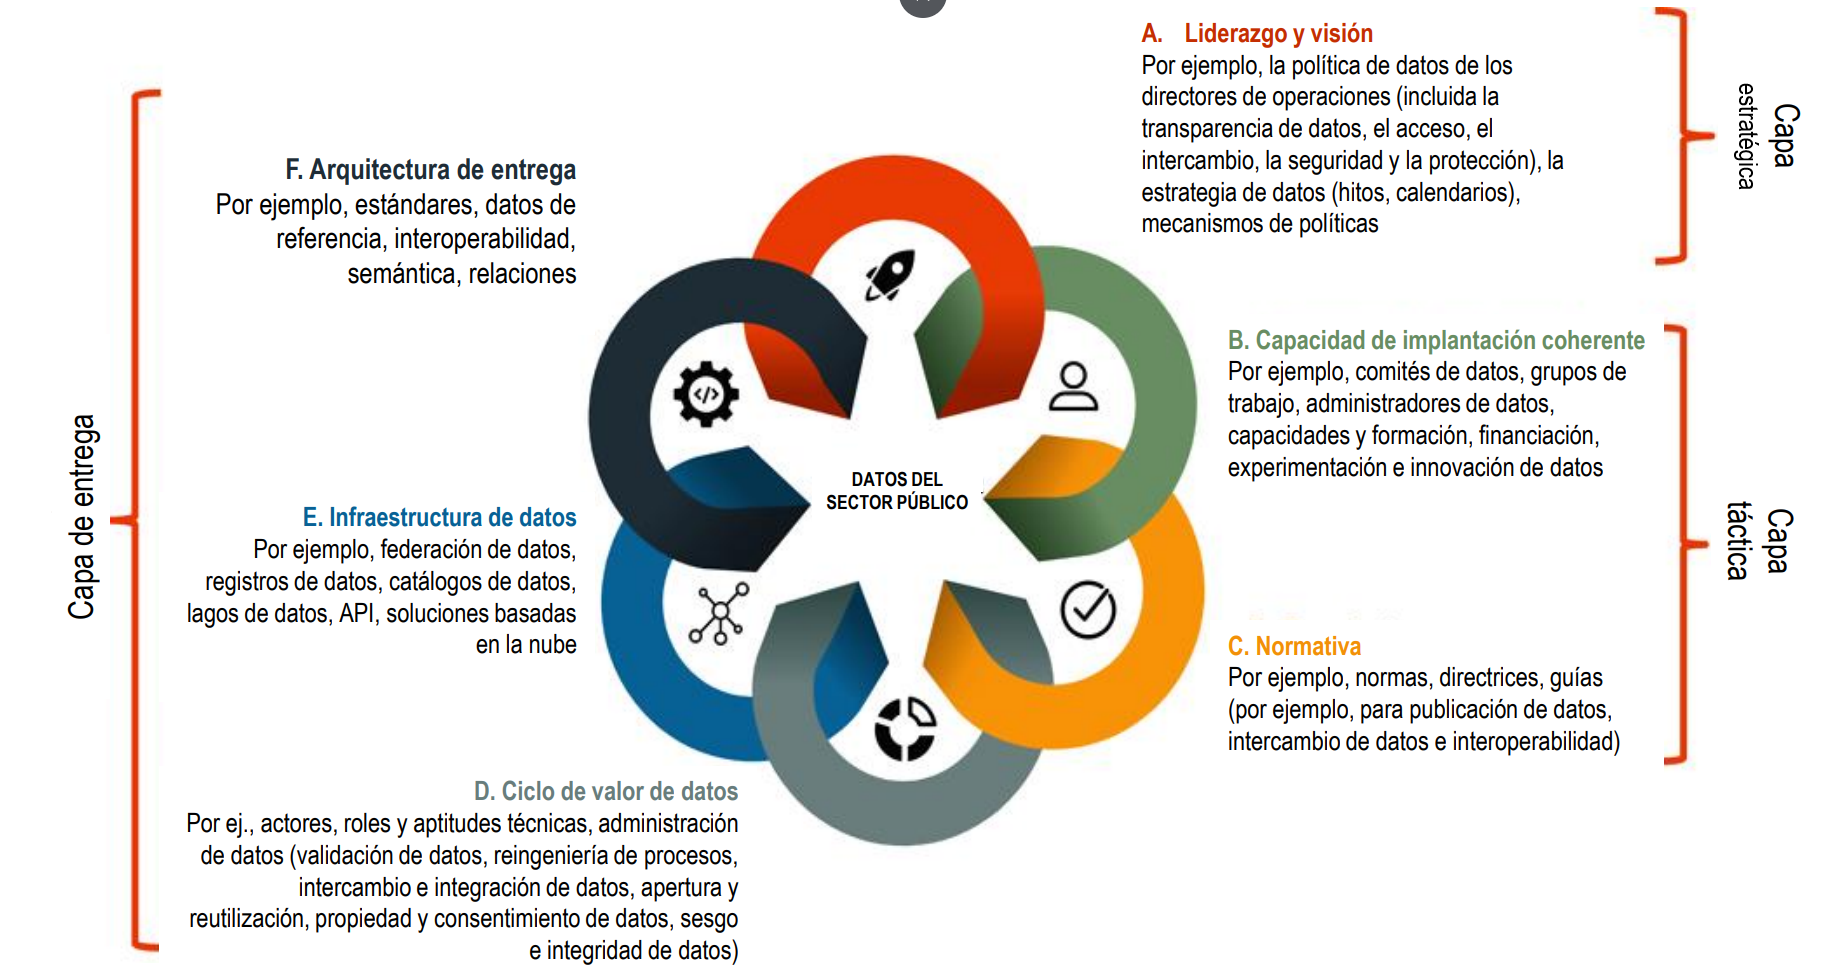
\includegraphics[scale=0.3]{Imagenes/Bitmap/data_gobernance.png} 
			\caption{Capas de gobierno del dato, fuente: \citep{OECD2019}.}
		\end{center}
	\end{figure}
	
	\newpage
	
	
	\subsection{Referente a Cloud}
	
	\item La \textbf{``Computación distribuida'' / ``Nube distribuida''} \label{def8} es un paradigma que aprovecha la capacidad de cálculo de miles o millones de dispositivos conectados a internet, creando una red de computación masiva, paralela y descentralizada. Los usuarios solo necesitan instalar un cliente de software que, cuando su dispositivo no está en uso, se encarga de descargar un pequeño fragmento de datos, procesarlo y devolver el resultado a un servidor central que coordina todas las tareas y ensambla los resultados finales. Este es un enfoque especialmente adecuado para problemas altamente paralelizables. Uno de los primeros productos en llevar la idea a cabo fue BOINC \citep{Anderson2004BOINC} para ayudar al cómputo de proyectos científicos. Actualmente, nubes como AWS o GCP se han apropiado del termino Nube distribuida, teniendo centros de datos en diferentes localizaciones para distribuir su trabajo a localizaciones mas cercanas o llevar la propia infraestructura y servicios de la nube fuera de sus data centres \citep{distributedGCP}.
	Esta idea evolucionó hasta la llamada ``Computación Voluntaria'' \citep{Anderson2010Volunteer}, donde dispositivos personales de voluntarios se usaban para este fin (ahora BOINC, cuyo software aún está disponible seria considerado computación voluntaria), y también se puede considerar que este paradigma se usa de forma malintencionada con varios casos famosos de ataques DDoS distribuidos \citep{MydoomDDoSMalware}, \citep{12Botnets} que usan dispositivos infectados para conseguir su propósito.
	
	También han surgido modelos con estas ideas paradigmas como el ``Dew computing'' \citep{DewComputing2018} donde los dispositivos personales se usan como almacenamiento, o plataformas de ``fog computing'' (que añade dispositivos intermedios en el calculo centralizado) o ``edge computing'' (Que ejecuta directamente en dispositivos finales) como SONM \citep{SONMWhitepaper} o otros proyectos \citep{BlockchainBasedDecentralisedCloud2018} que surgieron con el auge de las ``Blockchains'' y las usaban para poner en contacto usuarios que quisieran proporcionar potencia de cálculo con quienes querían usarla. En la actualidad, hay nubes que siguen activas como \citep{GolemNetwork}, \citep{akashCloud} ó \citep{rendernetwork} y que permiten comprar y vender potencia de cómputo.
	
	En resumen, todo lo englobado a la computación distribuida que hemos comentado se puede ver en esta tabla:
	
	\begin{table}[h]
		\centering
		\begin{tabular}{|p{0.15\textwidth}|p{0.55\textwidth}|p{0.30\textwidth}|}
			\hline
			\textbf{Modelo} & \textbf{Descripción} & \textbf{Ejemplo destacado} \\ \hline
			Nube distribuida & Infraestructura descentralizada, extendiendo servicios hacia el edge o centros locales. & Gestión centralizada con despliegue en edge/localización (AWS CloudFront, Google Cloud CDN). \\ \hline
			Computación voluntaria & Uso de recursos ociosos de dispositivos personales para cómputo distribuido voluntario. & BOINC, SETI@home, HTCondor, Techila Grid. \\ \hline
			``Dew Computing'' & Combina almacenamiento local y en la nube, sincronizando datos y permitiendo disponibilidad offline. & Dropbox. \\ \hline
			``Fog Computing'' & Procesamiento intermedio entre dispositivos y la nube, reduciendo latencia y uso de ancho de banda. & Aplicaciones IoT y casos de baja latencia / Vehículos autónomos. \\ \hline
			``Edge Computing'' & Procesamiento en dispositivos finales, priorizando latencia y seguridad. & Procesamiento de vídeo en tiempo real, reconocimiento facial en dispositivos móviles. \\ \hline
			``BotNets'' & Redes de dispositivos comprometidos que realizan tareas maliciosas de forma distribuida, usando el mismo principio de cómputo compartido pero con fines ilícitos. & Ataques DDoS (Mydoom), spam masivo, minería de criptomonedas no autorizada. \\ \hline
		\end{tabular}
		\caption{Comparación de modelos relacionados con la computación distribuida.}
		\label{tab:nube_distribuida}
	\end{table}
	
	\newpage %[TODO] revisar si quitar al final
	
	\item La \textbf{clasificación de la Computación en Nube} \label{def9} típicamente se puede dividir según dos dimensiones principales \citep{huawei2023cloud}:
	
	\textbf{Por modelo de operación:}
		\begin{itemize}
			\item \textbf{Nube Pública:} Infraestructura compartida y gestionada por proveedores externos (ej. AWS, Azure, Google Cloud), la cual ofrece acceso universal mediante pago por uso.
			\item \textbf{Nube Privada:} Infraestructura exclusiva para una organización, gestionada interna o externamente, y que tiene mayor control y seguridad.
			\item \textbf{Nube Comunitaria:} Compartida por varias organizaciones con intereses comunes (ej. instituciones académicas), y que presenta un equilibrio entre control y costes.
			\item \textbf{Nube Híbrida:} Combina nubes públicas y privadas, permitiendo mover cargas de trabajo según necesidades de seguridad, coste o escalabilidad.
			\item \textbf{Nube Industrial:} Especializada en sectores específicos (sanidad, automoción), con componentes optimizados para casos de uso particulares.
		\end{itemize}
		
		\textbf{Por modelo de servicio:}
		\begin{itemize}
			\item \textbf{IaaS (Infraestructura como Servicio):} Proporciona recursos fundamentales (máquinas virtuales, almacenamiento, redes). Ej: Amazon EC2, Google Compute Engine.
			\item \textbf{PaaS (Plataforma como Servicio):} Ofrece entornos de desarrollo y ejecución para aplicaciones. Ej: Google App Engine, Microsoft Azure App Services.
			\item \textbf{SaaS (Software como Servicio):} Software completo gestionado por el proveedor y accesible vía web. Ej: Gmail, Salesforce, Office 365.
		\end{itemize}
		
		En la \hyperref[figura_A2]{Figura \ref*{figura_A2}} se pueden observar una tabla que simplifica todos estos modelos de cloud por servicio.
		
		\begin{figure}[h]
			\begin{center}
				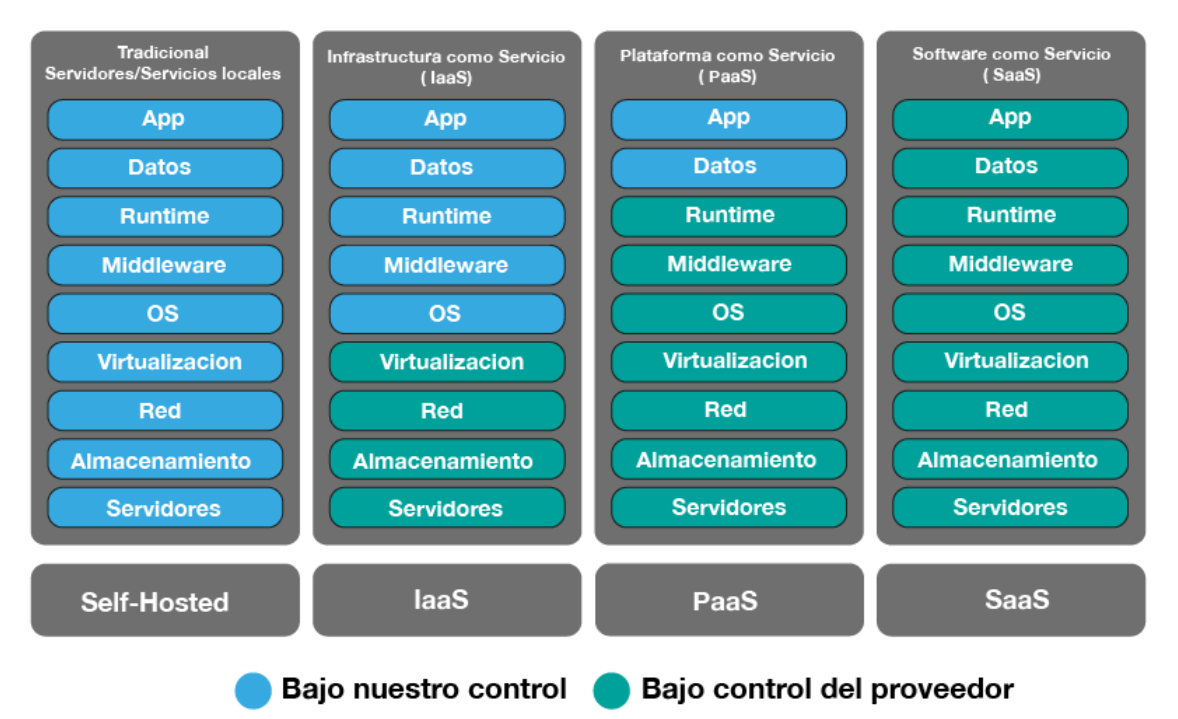
\includegraphics[scale=0.5]{Imagenes/Bitmap/distintos_tipos_clouds.png} 
				\caption{Distintos tipos de cloud, fuente: \citep{cloudPizza2014}.}
				\label{figura_A2}
			\end{center}
		\end{figure}
				
		\newpage %[TODO] revisar si quitar al final
		
		\item La \textbf{``Arquitectura en medalla''} \label{def11} es un patrón de diseño utilizado para gestionar el ciclo de vida de los datos en plataformas de datos, esta organiza y transforma datos en capas sucesivas: Bronce, Plata y Oro, y cada capa representa un nivel creciente de calidad y utilidad de los datos. Permite estructurar los datos para facilitar su ingestión, limpieza, enriquecimiento, análisis y consumo empresarial \citep{MedallionMicrosoft}. 
		Aunque lo hemos definido este nombre, quizás al lector le sea más familiar otra forma de procesar datos en capas \citep{MedallionMedium}, ya que la idea no es nueva en la ingeniería de datos y muchas otras metodologías introducen conceptos similares:
		\begin{itemize}
			\item \textbf{Arquitectura Clásica de Data Warehouse (Inmon):}
			\begin{itemize}
				\item Staging Area (Etapa de Carga) $\approx$ Capa Bronze
				\item CIF (Corporate Information Warehouse) $\approx$ Capa Silver
				\item Data Marts (Almacenamiento de Industria) $\approx$ Capa Gold
			\end{itemize}
			\item \textbf{``Data Vault'':}
			\begin{itemize}
				\item Staging Layer para procesamiento de flujos crudos $\approx$ Capa Bronze
				\item Raw Vault (donde se almacenan los datos originales) $\approx$ Capa Silver
				\item Business Vault o Data Marts (transforman datos en métricas) $\approx$ Capa Gold
			\end{itemize}
			\item \textbf{Data Mesh (Concepto de Propiedad de Datos Distribuida):}
			\begin{itemize}
				\item Raw Domain Data $\approx$ Capa Bronze
				\item Aggregated Domain Data $\approx$ Capa Silver
				\item Consumer-Oriented Products $\approx$ Capa Gold
			\end{itemize}
			\item \textbf{Patrón ``Write-Audit-Publish'':}
			\begin{itemize}
				\item Write (recolección de datos) $\approx$ Capa Bronze
				\item Audit (limpieza y procesamiento de datos) $\approx$ Capa Silver
				\item Publish (preparación para el uso) $\approx$ Capa Gold
			\end{itemize}
		\end{itemize}
		
		\newpage
		
		
	\subsection{Referente a Inteligencia Artificial}
		
	\item La \textbf{``Historia de la Inteligencia Artificial''} \label{def12} se remonta a hace casi un siglo, con la ideas de matemáticos como Alan Turing, que sentó las bases de la computación y propuso el primer test para evaluar inteligencia artificial \citep{Cheok2023AIHistory}. A partir de ese punto, no han parado de surgir avances en métodos matemáticos y algoritmos impulsando la búsqueda e implementación de modelos prácticos. Hitos como el desarrollo del perceptrón \citep{rosenblatt1958perceptron}, un modelo esencial para las redes neuronales; las cadenas de Markov, usadas como modelos estadísticos (Hidden Markov Model (HMM)); o el desarrollo del ``backpropagation'' que sentó las bases para que el entrenamiento de redes neuronales profundas fuera efectivo \citep{Werbos1974Backpropagation}. 
	
	Los avances, junto con el aumento de la computación siguiendo la ley de Moore, permitió el surgimiento y aumento de las redes neuronales recurrentes \citep{Hopfield1984RNN}, así como su uso para aplicaciones de procesamiento del lenguaje natural \citep{bengio2003neural}. Otro punto de inflexión lo puso Google con su articulo ``Attention Is All You Need'' \citep{vaswani2017attention}, donde definía que lo único que se necesitaba para procesar secuencias de forma eficaz era un mecanismo de atención, eliminando la necesidad de recurrencia y convoluciones, lo que permitió entrenar modelos más potentes sobre conjuntos de datos masivos, sentando las bases técnicas para los Grandes Modelos de Lenguaje (LLMs) como BERT o la serie GPT (Transformadores Pre-entrenados Generativos). 
	
	Tomando esta tecnología de los transformers, ``OpenAI'' lanzo diferentes versiones de su modelo GPT hasta culminar con una una interfaz conversacional basada en su modelo GPT-3,: ChatGPT. Esta interfaz se convirtió en una revolución, impulsando un interés público sin precedentes y consolidado a la IA como una herramienta indispensable. En los últimos años han seguido surgiendo modelos con tecnologías como la multimodalidad, donde los agentes combinan el procesamiento de texto escrito con otras fuentes como audio y visión en tiempo real, o el ``Mixture of experts (MoE)'' \citep{Jiang2024Mixtral} donde el modelo utiliza una combinación de múltiples redes neuronales (expertos), activando selectivamente un subconjunto de ellas para procesar cada entrada. Esta explosión en la presencia de la IA en la vida cotidiana, también ha impulsado, sobre todo en Europa, el desarrollo de marcos regulatorios para garantizar un uso responsable y transparente de estas tecnologías \citep{webRIA2024Europa}.
	
	\emph{Matiz: Si bien tecnologías de visión por computador o generación de multimedia son pilares fundamentales de la IA moderna y cruciales para los LLMs multimodales, es necesario acotar el alcance de este trabajo. Por lo tanto, esta definicion se centra en los avances relacionados con el procesamiento de datos estructurados y texto, dejando fuera un análisis detallado del tratamiento específico de vídeo, audio e imagen, a pesar de reconocer su enorme relevancia e impacto.}
		
		
	Para facilitar la visualización de esta definición, resumiremos los hitos que consideramos importantes en orden cronológico:
	\begin{table}[h]
		\centering
		\begin{tabular}{@{}r@{\hspace{1em}}|@{\hspace{1em}}p{11cm}@{}}
			\multicolumn{2}{@{}c@{}}{\textbf{Línea de tiempo de IA}} \\ \\
			1936 & \textbf{Turing machines} - Marco teórico para computación \\
			1950 & \textbf{Turing test} - Primera medida práctica de inteligencia máquina \\
			1958 & \textbf{Perceptrón} - Modelo base de las redes neuronales \\
			1964 & \textbf{ELIZA} - Primer chatbot conversacional \\
			1966 & \textbf{Hidden Markov Model} - Modelo estadístico temprano \\ 
			1967 & \textbf{K-means} - Algoritmo popular de clustering \\
			1974 & \textbf{Backpropagation} - Algoritmo fundamental para ANN multicapa \\	
			1982 & \textbf{RNN} - Redes neuronales recurrentes\\
			1997 & \textbf{LSTM} - RNN con memoria a largo plazo \\
			\    & \textbf{Deep Blue} vence a Kasparov \\
			2003 & \textbf{NPLM} Aprendizaje de "embeddings" de palabras, base de  LLM \\
			2014 & \textbf{GAN} - Generación de datos nuevos \\
			2016 & \textbf{AlphaGo} - Derroto al campeón del mundo \\
			2017 & \textbf{Transformers} - Arquitectura basada en atención \\
			2018 & \textbf{BERT}, \textbf{GPT-1} - Modelos de lenguaje grandes (LLM) \\
			2020 & \textbf{GPT-3} - aumento de las capacidades y parámetros \\
			2021 & \textbf{DALL-E} - Imágenes desde texto \\
			2022 & \textbf{ChatGPT} - Interfaz conversacional, aumenta el interés publico \\
			2023 & \textbf{GPT-4} - Modelo multimodal \\
			\    & \textbf{LLaMA} Modelo Open-Source \\
			2024 & \textbf{GPT-4o} - Modelo multimodal con voz y visión en tiempo real \\
			\    & \textbf{EU AI Act} - Regulación integral sobre IA \\
			2025 & \textbf{DeepSeek} - LLM de bajo costo \\
			\    & \textbf{IA Agéntica y especializada} - agentes autónomos, tareas específicas \\
		\end{tabular}
		\caption{Fuente: Adaptación y actualización de \citep{Cheok2023AIHistory}, complementada con información de \citep{Sapkota2025Agentic}, \citep{Bit2BrainHistoriaIA}, \citep{Campbell2002DeepBlue} y las referencias mencionadas en el texto.}
	\end{table}
	
	\newpage %[TODO] ver si es necesario al final
	
	Como frase final, y espero que esperanzadora, incluir que a pesar de que esta tecnología ha pasado por algunas épocas de menor interés publico, los datos de Web parecen mostrar que esta vez la tecnología viene para quedarse [Figura \ref{figura_A3}]. Ya que a pesar de que un ultimo estudio del MIT anuncia que el 95\% de los proyectos con IA reciben retorno cero \citep{challapally2025state}, diversos analistas sostienen que esto no implica una burbuja vacía, sino más bien una fase inicial en la que muchos pilotos fracasaran por problemas de integración o organizativos y no por fallos tecnológicos. Al igual que ocurrió con la burbuja de las dot.com, de la cual emergieron gigantes como Amazon y Google, se espera que también en IA sobrevivan los proyectos con verdadero valor \citep{Video_AIExplained_AIBubble_2025}.
	
	\begin{figure}[h]
		\begin{center}
			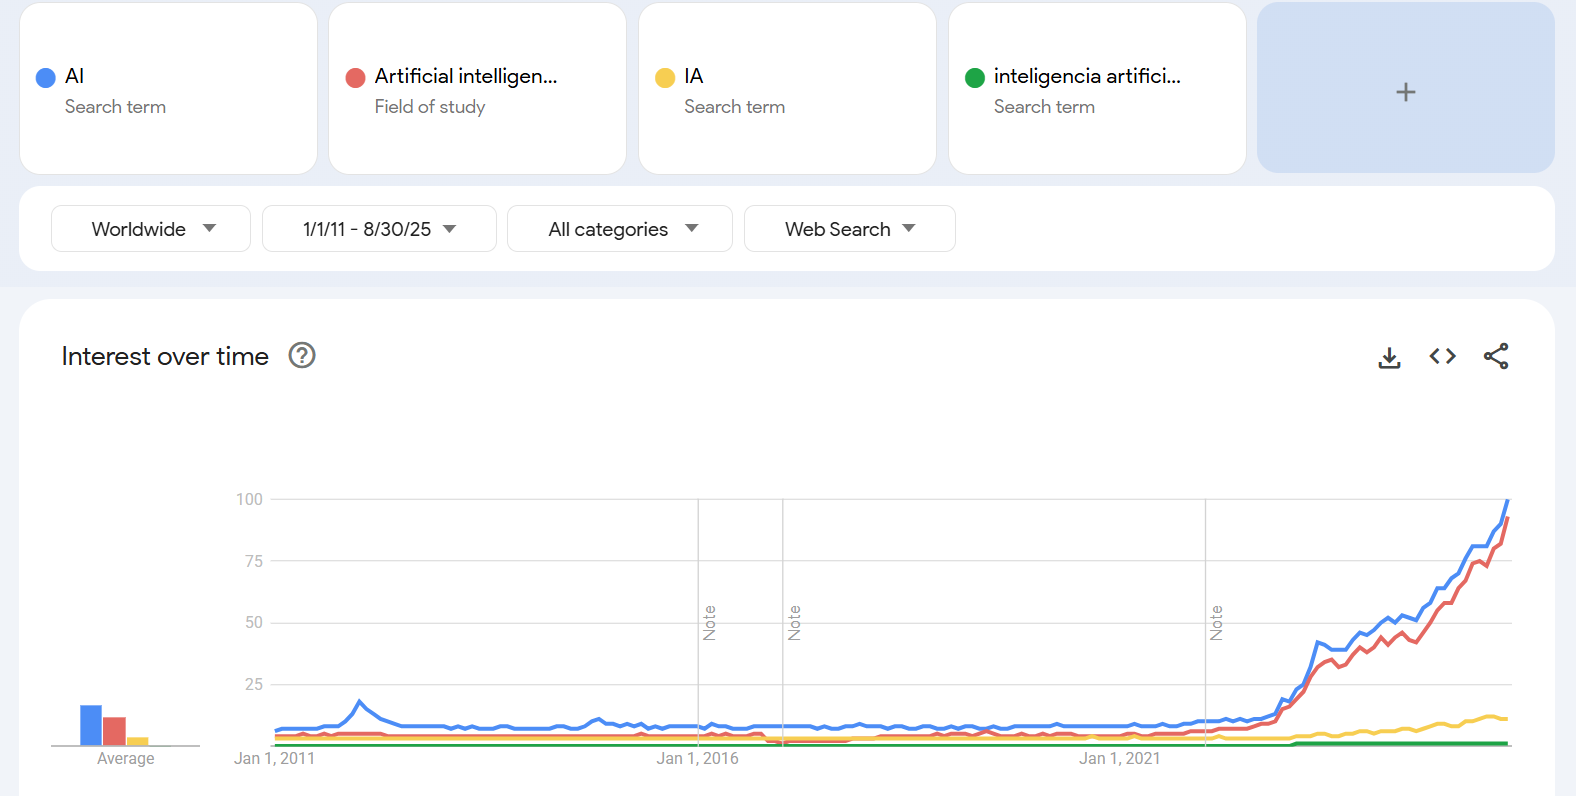
\includegraphics[scale=0.3]{Imagenes/Bitmap/IA_Trends2011_2025.png} 
			\caption{Tendencias de búsqueda de IA: \citep{TrendsGoogleIA2025},	\emph{Destacar el pico de 2011 por el lanzamiento de Siri (Apple) y la tendencia desde 2022 por la salida de chatGPT.}} 
			\label{figura_A3}
		\end{center}
	\end{figure} 
	
	\vspace{1cm}
	
	\item Los tipos de \textbf{Técnicas de ML según aprendizaje} \label{def13} es la forma de clasificar estos modelos dependiendo de la forma en la que los sistemas aprenden patrones, o del grado de supervisión que reciben. Se clasifican en cuatro tipos principales \citep{Sarker2021}: 
	\begin{itemize}
		\item \textbf{Aprendizaje Supervisado:} utiliza datos etiquetados para aprender una función que mapea entradas a salidas. Esta orientada a tareas concretas, y sus aplicaciones más comunes incluyen clasificación y regresión, como predecir la cantidad de ventas de un producto. 
		
		\item \textbf{Aprendizaje No Supervisado:} analiza datos no etiquetados, buscando estructuras, patrones o relaciones ocultas. Es un enfoque orientado al descubrimiento y exploración, y se aplica típicamente en clusterización, reducción de dimensionalidad o detección de anomalías. 
		
		\item \textbf{Aprendizaje Semi-Supervisado:} combina datos etiquetados y no etiquetados, aprovechando la abundancia de datos sin etiqueta para mejorar el rendimiento del modelo más allá de lo que se lograría solo con datos etiquetados. Es útil en contextos donde las etiquetas son costosas o escasas, como en detección de fraude o clasificación de texto. 
		
		\item \textbf{Aprendizaje por Refuerzo:} se basa en la interacción de un agente con un entorno, aprendiendo mediante recompensas o penalizaciones para optimizar su comportamiento. Se aplica en tareas de automatización compleja y optimización, como robótica o conducción autónoma. \\ \\ 
	\end{itemize}
	
	\item  \textbf{MLOps} \label{def14} u operaciones de aprendizaje automático, son un conjunto de prácticas y herramientas que busca automatizar y gestionar el ciclo de vida completo de un proyecto de machine learning, desde el desarrollo del modelo hasta su despliegue, monitoreo y mantenimiento en producción, basándose en principios de DevOps pero adaptados a las particularidades de los sistemas de ML \citep{Kreuzberger2023MLOps}. Los nueve principios son los siguientes:
	\begin{enumerate}
		\item \textbf{Automatización CI/CD:} Integración, entrega y despliegue continuos que automatizan el desarrollo, prueba y puesta en producción de los modelos, proporcionando información rápida sobre el éxito o fracaso de cada paso.
		
		\item \textbf{Orquestación del flujo de trabajo (workflow):} Coordinación y gestión de las tareas de un ``pipeline'' o proceso de ML, estableciendo el orden de ejecución y dependencias, típicamente mediante DAGs.
		
		\item \textbf{Reproducibilidad:} Capacidad fundamental de replicar el experimento de ML y obtener los mismos resultados.
		
		\item \textbf{Control de versiones:} Implica la gestión y el seguimiento riguroso de los cambios en los datos, modelos y código (indispensable para la trazabilidad y el cumplimiento normativo).
		
		\item \textbf{Colaboración:} Promueve el trabajo conjunto y una cultura comunicativa y abierta entre los diferentes roles del proyecto para minimizar aislamiento de datos e información.
		
		\item \textbf{Entrenamiento y evaluación continuos:} Implica el retrenamiento periódico y automático de los modelos con nuevos datos, incluyendo una evaluación constante de su calidad para asegurar que sigan siendo relevantes, precisos y óptimos en cuanto a rendimiento.
		
		\item \textbf{Seguimiento y registro de metadatos:} Documentación detallada de la información relevante de cada ejecución del flujo para asegurar trazabilidad: parámetros utilizados, métricas, código, tiempo de ejecución y los datos utilizados.
		
		\item \textbf{Monitoreo continuo:} Observación periódica de los datos, modelos, código, infraestructura y rendimiento del modelo desplegado, con el objetivo de detectar anomalías, errores o bajadas en la calidad.
		
		\item \textbf{Bucles de retroalimentación:} Integrar los hallazgos y las lecciones aprendidas del monitoreo y la evaluación de calidad en el proceso de desarrollo.  \\ \\ 
		
		
	\item \textbf{Modelos de Machine learning}.  \label{def15} Estas definiciones se basan en el curso de \citep{JasonMachinelearningmastery}, el libro del mismo autor \citep{Brownlee_2016_MLAFS} y en los libros \citep{Fowdur2021} y \citep{Sarker2021}, así como en la asignatura ``desarrollo de aplicaciones y servicios inteligentes'' impartida por la Universidad Complutense de Madrid. Aunque para estas definiciones \textbf{no} nos centraremos en como efectuar la selección de hiperparámetros (parámetros externos al modelo que lo configuran), nombrar que el rendimiento y complejidad de estos modelos depende de la correcta elección de esta característica. También, por alcance, detallaremos solo los modelos que se han elegido para estudiar en este de entre la gran variedad de ellos que existe \citep{MachineLearningMethodsList}, estos son los siguientes:
	
	\begin{enumerate}
		\item \textbf{Árboles de Decisión (Decision Trees):}
		Son un método de aprendizaje \textbf{supervisado} no paramétrico utilizado para \textbf{clasificación y regresión}. Consiguen su objetivo dividiendo recursivamente el conjunto de datos de entrenamiento en subconjuntos más pequeños, evaluando todas las posibles divisiones en cada característica de entrada para encontrar el punto de división óptimo que minimice la función de coste. El proceso continúa hasta alcanzar un criterio de detención, obteniendo los nodos terminales que contienen la predicción final (la clase más común o el promedio de valores).
		
		\item \textbf{k-Nearest Neighbors (k-NN):}
		Es un algoritmo de aprendizaje \textbf{supervisado} de "aprendizaje perezoso" (no ejecuta hasta que no se le pida una predicción), utilizado para \textbf{clasificación y regresión}. Consigue su objetivo para nuevos datos calculando la distancia entre este y todos los ejemplos del conjunto de entrenamiento. Luego, selecciona los \emph{k} ejemplos más parecidos (vecinos). Para clasificación, la predicción es la clase más común entre estos \emph{k} vecinos; para regresión, es el promedio de sus valores de salida.
		
		\item \textbf{K-means:}
		Es un algoritmo de aprendizaje \textbf{no supervisado} utilizado para la \textbf{clusterización}. Consigue su objetivo al identificar \emph{k} centroides en el conjunto de datos y luego asigna cada punto de datos al centroide más cercano durante varias iteraciones, estos centroides se actualizan continuamente moviéndose al promedio de todos los puntos asignados a su cluster, y despues de esto los puntos se reasignan, con el fin de minimizar la suma de las distancias cuadradas entre cada punto de datos y su centroide asignado.
		
		\item \textbf{Random Forests (Bosques Aleatorios):}
		Es un método de ensamble de aprendizaje supervisado utilizado para clasificación y regresión. Consigue su objetivo construyendo un "bosque" de múltiples árboles de decisión individuales. Cada árbol se entrena en una submuestra aleatoria del conjunto de datos con reemplazo (bagging), y en cada punto de división se considera solo un subconjunto aleatorio de características. Las predicciones finales se obtienen combinando las predicciones de todos los árboles del bosque: por votación mayoritaria para clasificación o por promedio para regresión, lo que reduce la varianza y mejora la precisión.
		
		\item \textbf{XGBoost (Extreme Gradient Boosting):}
		Es una implementación optimizada y escalable de algoritmos de ``gradient boosting'', un método de ensamble de aprendizaje \textbf{supervisado para clasificación y regresión}. Consigue su objetivo construyendo una serie de modelos individuales de forma secuencial (normalmente árboles de decisión), donde cada nuevo modelo se entrena para corregir los errores residuales de los árboles previos. Para ello, minimiza una ``función de pérdida'' que cuantifica el error del modelo empleando aproximaciones de segundo orden. Esto significa que, computa tanto la pendiente de la función de pérdida (como en el descenso de gradiente básico) como su curvatura para encontrar el mínimo, lo que resulta en una convergencia más rápida y una mayor exactitud. Además, aplica técnicas de regularización avanzadas (L1 y L2) para prevenir el sobre-ajuste y mejorar la generalización. La regularización L1 (Lasso) penaliza la suma de los valores absolutos de los coeficientes, pudiendo llevar algunos a cero y realizando selección de características; la regularización L2 (Ridge) penaliza la suma de los cuadrados de los coeficientes, reduciéndolos sin eliminarlos.
		
		\item \textbf{DBSCAN:}
		Es un algoritmo de aprendizaje \textbf{no supervisado para clusterización} basado en ``densidad''. Consigue su objetivo identificando regiones densas de puntos de datos separadas por regiones de menor densidad, clasificando los puntos como centrales, frontera o de ruido, y forma cada clúster a partir de puntos que están densamente conectados. No requiere que se especifique el número de clústeres de antemano y es capaz de descubrir clústeres de formas arbitrarias, además de identificar valores extremos.
		
		\item \textbf{Redes Neuronales Profundas (Deep Neural Networks - DNN):}
		Brevemente, son modelos de aprendizaje \textbf{supervisado} que incluyen arquitecturas como los perceptrones multicapa (MLP). Consiguen su objetivo aprendiendo representaciones jerárquicas de los datos a través de múltiples capas ocultas de procesamiento (capas ocultas). El proceso de entrenamiento implica la propagación hacia adelante de la entrada para calcular una salida, seguida de la retropropagación ("Backpropagation") del error para ajustar iterativamente los pesos de las conexiones, minimizando la diferencia entre la salida predicha y la esperada. Son aptas para \textbf{clasificación y regresión en datos complejos}. \cite{Brownlee2018, Sarker2021}
		
		\item \textbf{Grandes Modelos de Lenguaje (Large Language Models - LLM):}
		Son un tipo avanzado de Redes Neuronales Profundas, frecuentemente basadas en la arquitectura de ``transformers''. Consiguen su objetivo mediante un pre-entrenamiento masivo en vastos corpus de texto y código, permitiendo aprender patrones complejos de lenguaje, gramática, semántica y contextualización. Su mecanismo de atención les permite ponderar la importancia de diferentes partes de la entrada, facilitando una comprensión profunda y la generación de texto coherente y relevante. Se utilizan para una amplia gama de tareas de procesamiento de lenguaje natural (PNL). \cite{Sarker2021}    \\ \\ 
	\end{enumerate}

	\item 
	\end{enumerate}
	
\end{enumerate}
\newpage

\section{Acrónimos}
\label{sec:acronimos}

\begin{description}
	
	\item[AI] Inteligencia Artificial (Artificial Intelligence)
	\item[AI Act] Ley de Inteligencia Artificial (Artificial Intelligence Act)
	\item[ANN] Redes Neuronales Artificiales (Artificial Neural Network)
	\item[API] Interfaz de Programación de Aplicaciones (Application Programming Interface)
	\item[ARIMA] Modelo Autorregresivo Integrado de Medias Móviles (Autoregressive Integrated Moving Average)
	\item[AWS] Amazon Web Services
	\item[BDTI] Big Data Test Infrastructure
	\item[BERT] Representaciones de Codificador Bidireccional de Transformadores (Bidirectional Encoder Representations from Transformers)
	\item[BOINC] Berkeley Open Infrastructure for Network Computing
	\item[BTOS] Encuesta sobre Tendencias y Panorama Empresarial (Business Trends and Outlook Survey)
	\item[CCPA] Ley de Privacidad del Consumidor de California (California Consumer Privacy Act)
	\item[CDN] Red de Distribución de Contenidos (Content Delivery Network)
	\item[CI/CD] Integración Continua/Entrega Continua (Continuous Integration/Continuous Delivery)
	\item[CIF] Corporate Information Warehouse
	\item[CKAN] Comprehensive Knowledge Archive Network
	\item[CNN] Red Neuronal Convolucional (Convolutional Neural Network)
	\item[CNMC] Comisión Nacional de los Mercados y la Competencia
	\item[CPU] Unidad Central de Procesamiento (Central Processing Unit)
	\item[CSV] Valores Separados por Comas (Comma-Separated Values)
	\item[D1] D1 Database (Base de datos de Cloudflare)
	\item[DAGs] Grafos Acíclicos Dirigidos (Directed Acyclic Graphs)
	\item[DBSCAN] Clustering Espacial Basado en Densidad de Aplicaciones con Ruido (Density-Based Spatial Clustering of Applications with Noise)
	\item[DDoS] Ataque de Denegación de Servicio Distribuido (Distributed Denial of Service)
	\item[DevOps] Development and Operations
	\item[DNN] Redes Neuronales Profundas (Deep Neural Networks)
	\item[DNS] Sistema de Nombres de Dominio (Domain Name System)
	\item[DSL] Ley de Seguridad de Datos (Data Security Law) - China
	\item[EC2] Elastic Compute Cloud (Amazon EC2)
	\item[EEUU] Estados Unidos
	\item[EU] European Union (Unión Europea)
	\item[GAN] Red Generativa Antagónica (Generative Adversarial Network)
	\item[GCP] Google Cloud Platform
	\item[GPT] Transformador Pre-entrenado Generativo (Generative Pre-trained Transformer)
	\item[GPU] Unidad de Procesamiento Gráfico (Graphics Processing Unit)
	\item[HIPAA] Ley de Portabilidad y Responsabilidad de Seguros de Salud (Health Insurance Portability and Accountability Act)
	\item[HITL] Human in the loop (mantener al humano en los procesos (blucles) de Inteligencia artificial)
	\item[HMM] Modelo Oculto de Markov (Hidden Markov Model)
	\item[HTTP] Hypertext Transfer Protocol
	\item[IA] Inteligencia Artificial (Artificial Intelligence)
	\item[IaaS] Infraestructura como Servicio (Infrastructure as a Service)
	\item[IBM] International Business Machines (empresa)
	\item[IDE] Entorno de Desarrollo Integrado (Integrated Development Environment)
	\item[INE] Instituto Nacional de Estadística
	\item[IoT] Internet de las Cosas (Internet of Things)
	\item[IP] Internet Protocol
	\item[IPv4] Internet Protocol version 4
	\item[JSON] Notación de Objetos de JavaScript (JavaScript Object Notation)
	\item[k-NN] k-Nearest Neighbors (k-Vecinos Más Cercanos). Algoritmo de aprendizaje automático.
	\item[KV] Key-Value (Almacenamiento Clave-Valor)
	\item[LGD] Ley de Gobernanza de Datos
	\item[LLM] Modelo de Lenguaje a Gran Escala (Large Language Model)
	\item[LSTM] Memoria a Largo-Corto Plazo (Long Short-Term Memory)
	\item[MIT] Massachusetts Institute of Technology (Instituto de Tecnología de Massachusetts)
	\item[ML] Aprendizaje Automático (Machine Learning)
	\item[MLOps] Operaciones de Aprendizaje Automático (Machine Learning Operations)
	\item[MLP] Perceptrón Multicapa (Multi-layer Perceptron)
	\item[NLP] Procesamiento del Lenguaje Natural (Natural Language Processing)
	\item[NoSQL] Not only SQL
	\item[NPLM] Modelo de Lenguaje Neuronal Probabilístico (Neural Probabilistic Language Model)
	\item[OECD] Organización para la Cooperación y el Desarrollo Económicos (Organisation for Economic Co-operation and Development)
	\item[OGDA] Ley de Datos Abiertos del Gobierno (OPEN Government Data Act)
	\item[OKF] Open Knowledge Foundation
	\item[PaaS] Plataforma como Servicio (Platform as a Service)
	\item[PIPL] Ley de Protección de Información Personal (Personal Information Protection Law) - China
	\item[PLN] Procesamiento del Lenguaje Natural (Natural Language Processing)
	\item[R2] R2 Storage (Almacenamiento de Cloudflare)
	\item[RAM] Memoria de Acceso Aleatorio (Random Access Memory)
	\item[RL] Aprendizaje por Refuerzo (Reinforcement Learning)
	\item[RNN] Redes Neuronales Recurrentes (Recurrent Neural Network)
	\item[RGPD] Reglamento General de Protección de Datos
	\item[S3] Simple Storage Service (Amazon S3)
	\item[SaaS] Software como Servicio (Software as a Service)
	\item[SASE] Acceso Seguro al Borde del Servicio (Secure Access Service Edge)
	\item[SIMPL] Smart Middleware Platform for Cloud-to-Edge (EU)
	\item[SQL] Lenguaje de Consulta Estructurado (Structured Query Language)
	\item[SSL] Capa de Conexión Segura (Secure Sockets Layer)
	\item[SSD] Disco de Estado Sólido (Solid State Drive)
	\item[TPU] Unidad de Procesamiento Tensorial (Tensor Processing Unit)
	\item[TURN] Traversal Using Relays around NAT (Network Address Translation)
	\item[UE] Unión Europea
	\item[XLSX] Excel Open XML Spreadsheet
	
\end{description}


 \newpage
